
\subsectionfont{\fontsize{14}{14}\selectfont}
\graphicspath{{./images/}}


\subsection{Dashboard}
The user interface showcases a dashboard that displays real-time information about the rocket on the Home page. 
It features a "Satellites in View" container that displays satellites that are utilized by the rocket. 
It also contains various graphs that illustrate data received from the backend via a WebSocket. 
The "Satellites in View" and graphs are updated in real time to provide the user with an understanding 
of the rocket's current status. 

\begin{figure}[H]
    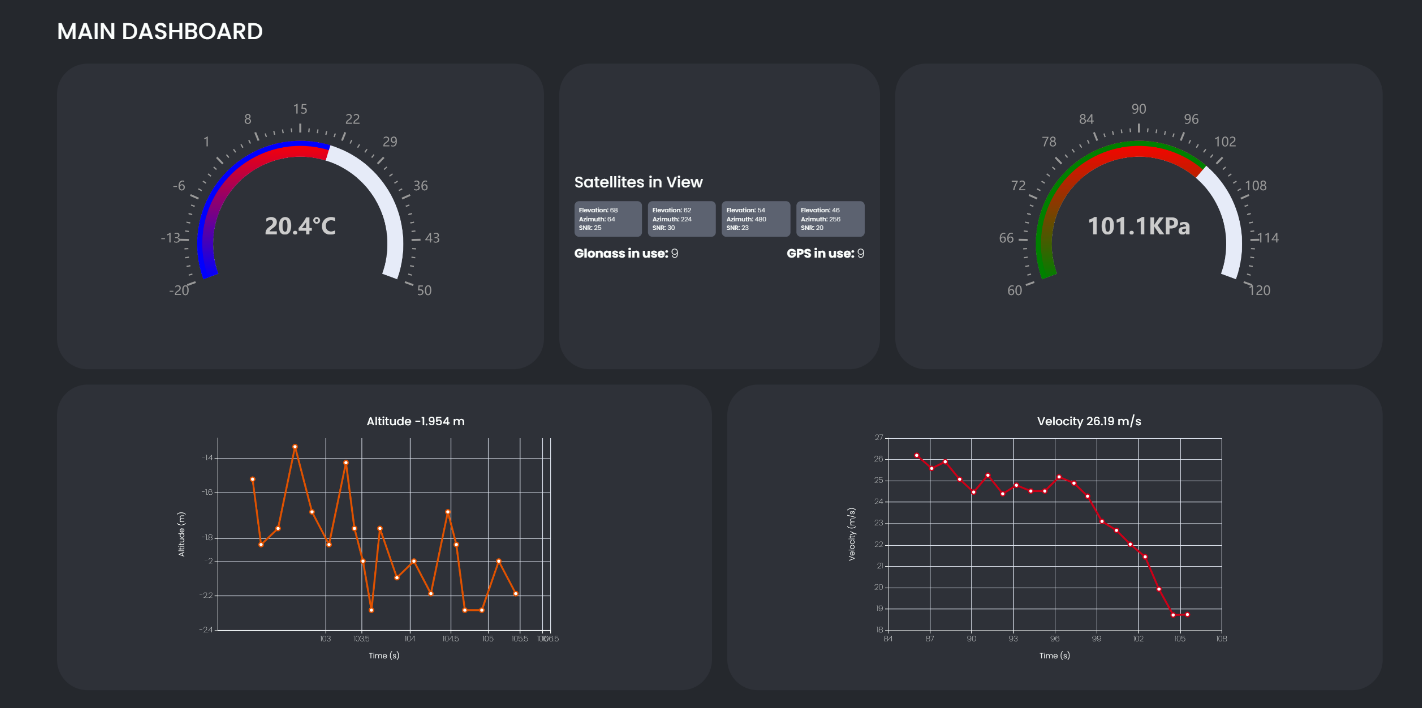
\includegraphics [scale=0.75] {ui_dashboard}
    \centering
    \captionof{figure} {The dashboard of the user interface}
\end{figure}

\subsubsection {Satellites in View}
The "Satellites in View" displays satellites that are being used by the GLONASS and GPS
navigation system to track the live location of the rocket. 
It shows the following information of the satellite:

\begin{itemize}
    \item \textbf{Elevation:} Represents the elevation of the satellite in degrees
    \item \textbf{Azimuth:} Represents the satellite azimuth in degrees
    \item \textbf{SNR:} Represents the signal to noise ratio from a satellite in dB Hz
\end{itemize}

\begin{figure}[H]
    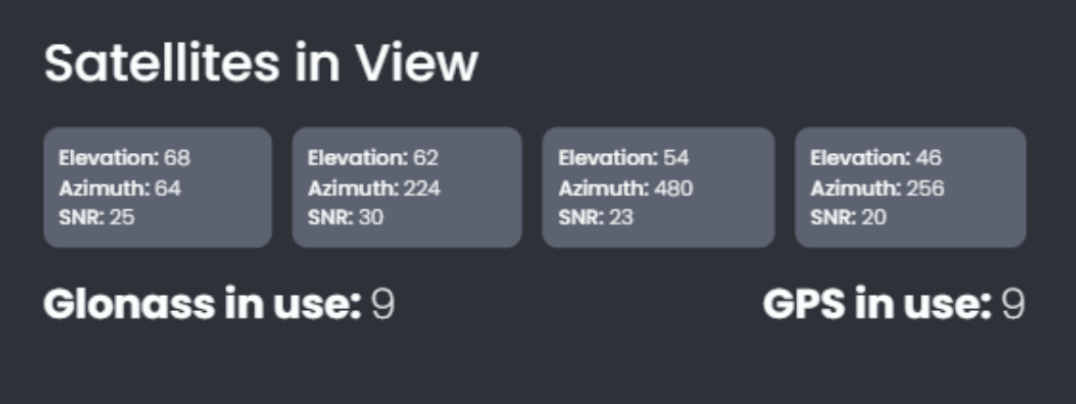
\includegraphics [scale=0.5] {ui_satellites_in_view}
    \centering
    \captionof{figure} {Satellites in View container in the dashboard}
\end{figure}

\subsubsection{Graphs}
The user interface displays two types of graphs: trend and gauge graphs. 
The type of graph used to display information depends on the nature of the data being represented. 
To display the graphs, the ReactECharts library was used to create two different JSX components: 
gauge graph and trend graph. The JSX graph components use the x and y packets of the data sent by the 
WebSocket to display the information. Each JSX graph component that is rendered to the Home page has 
props being passed to present the data in a clear and user-friendly format.
\footnote{Note: This is not an exhaustive list 
of props, but rather a selection of them}: 

\begin{multicols}{2}
    \begin{itemize} 
        \item title of the graph    
        \item units of the graph       
        \item colour theme of the graph
        \item title of the axis
        \item x values          
        \item y values
    \end{itemize}
\end{multicols}



\textbf{Trend Graphs}
\\Trend graphs are used to display data over a period of time and 
are best suited for showing changes in data over time. The dashboard used trend graphs
to represent velocity, acceleration and altitude over time. Each trend graphs has 
at least 10 points represented at any moment as the x and y packets are sent as an array of 10 values.

\begin{figure}[H]
    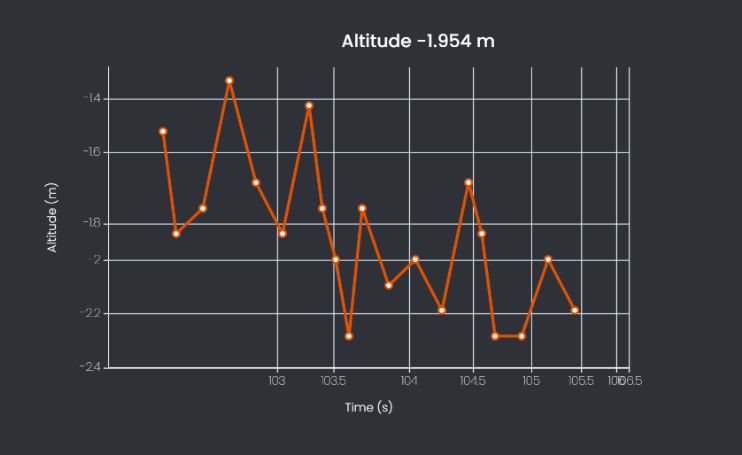
\includegraphics [scale=0.75] {ui_trend_graph}
    \centering
    \captionof{figure} {A trend graph displaying altitude over time of the rocket}
\end{figure}



\textbf{Gauge Graphs}
\\Gauge graphs are used to display a single value or data point at a specific moment in
time and are best suited for displaying real-time data for temperature and pressure. To specify a range for each
gauge meter, the maximum and minimum values are also passed into the Gauge graph component. The value 
displayed in the gauge meter is the last y value of the packet sent by the WebSocket to ensure the latest information
is presented. 


\begin{figure}[H]
    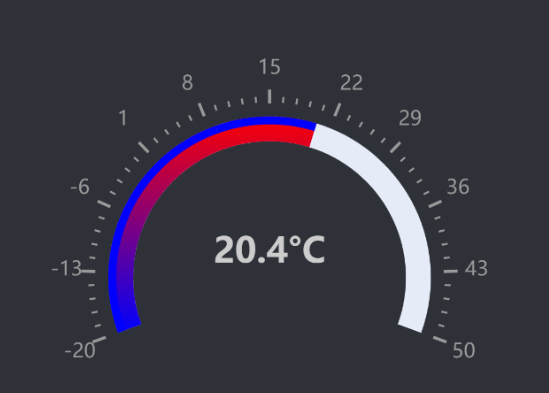
\includegraphics [scale=0.75] {ui_gauge_graph}
    \centering
    \captionof{figure} {A gauge graph displaying the temperature of the rocket}
\end{figure}

